\chapter{Background}
\label{ch:background}

% ``Everybody who learns concurrency thinks they understand it, ends up finding mysterious races they thought weren’t possible, and discovers that they didn’t actually understand it yet after all.'' -- Herb Sutter, chair of the ISO C++ standards committee, Microsoft.

The background for this project will provide a summary of relevant aspects of the Rust programming language and the field of \acrshort{HPC}, along with a literature review of existing performance analyses of Rust in \acrshort{HPC} applications.


\section{The Rust Language}
\label{sec:rust}

This section provides a description of salient features of the Rust language, which are required to understand the intricacies of the translation, equivalence checking, and performance analysis processes described in this project. Aspects of the content of this introduction are derived from Klabnik and Nichols' book ``The Rust Programming Language'' \cite{RustProgrammingLanguage}. This is the seminal text for beginners learning Rust, affectionately nicknamed ``the book'' within the Rust community \cite{LearnRust}.

\subsection{Basic syntax}
\label{ssec:rust-syntax}

In any programming language, the first program written tends to be printing ``Hello World'', a tradition introduced by Kernighan and Ritchie in the first chapter of ``The C Programming Language'' \cite{kernighan2002c}. In Rust, the ``Hello world'' program is shown in Listing \ref{listing:rust-hello-world}.

\begin{code}
    %TC:ignore
    \begin{minted}{rust}
        fn main() {
            println!("Hello, world!");
        }
    \end{minted}
    %TC:endignore
    \caption{Rust program to print ``Hello, world!'', derived from Listing 1-1 of ``The Rust Programming Language'' \cite{RustProgrammingLanguage}.}
    \label{listing:rust-hello-world}
\end{code}

The influence of the C-family of languages on Rust's syntax is clear, for example the use of braces and semicolons, along with the presence of a \mintinline{rust}{main} function.

% After having printed ``Hello World'', the next thing a programmer is likely to do in an imperative language is define a variable. However, this is where the influence of functional languages like Haskell and the ML-family begins to show -- variables in Rust are immutable by default. As chapter 3-1 of the Rust book states, this is ``one of the many nudges Rust gives you to write your code in a way that takes advantage of the safety and easy concurrency that Rust offers'' \cite{RustProgrammingLanguage}, since immutable variables are easier for the compiler to reason about to provide guarantees of memory safety.

% Variables in Rust are defined using the \mintinline{rust}{let} keyword, and can be explicitly marked as mutable when required using the \mintinline{rust}{mut} keyword. In addition to this, namespace shadowing can be used to redefine variables with new values, by re-using the \mintinline{rust}{let} keyword. Some of the semantics of Rust variables are shown in Listing \ref{}.

% % Type system
% Another aspect of Rust's pedigree from functional languages is its rich type system.

% % Iterators
% One of the many ergonomic features Rust provides is ``zero-cost abstractions''. This refers to high-level structures to perform common tasks, such as the \mintinline{rust}{fold} operation on vectors, which compiles down to the same, performant, assembly as a more verbose iterative expression of the same functionality. Zero-cost abstractions allow programmers to write terse code, whilst not sacrificing performance.

% One example of a zero-cost abstraction is Rust's iterators.


\subsection{Ownership model}
\label{ssec:rust-ownership}

As mentioned in the introduction, a core feature of Rust is its guarantees against undefined behaviour. These guarantees are provided in large part by its ownership model, enforced by an aspect of the compiler called the borrow checker \cite{ReferencesBorrowing}. Most languages employ one of two strategies for managing memory: garbage collection or manual memory management \cite{hertzQuantifyingPerformanceGarbage2005}. In garbage collected languages such as Java and Python, there is a runtime environment which executes alongside the program, allocating memory when required, and deallocating it when it is no longer in use. However, this additional overhead of the garbage collector running in parallel typically incurs a performance cost  \cite{hertzQuantifyingPerformanceGarbage2005}. In manual memory management, the allocation and deallocation of memory is explicitly controlled by the programmer. This avoids the runtime cost of the garbage collector, but can lead to errors and undefined behaviour if the programmer makes a mistake, such as double-free and use-after-free errors respectively.

Rust takes a third approach to memory management, enforcing a set of ownership rules checked by the compiler. By following these rules, the compiler can always infer when memory is no longer in use through scope or explicit lifetimes, and deallocate it as required. Furthermore, it provides strong guarantees against undefined behaviour as a result of invalid memory accesses and data races, since these are prohibited by the ownership rules. In ``The Rust Programming Language'' \cite{RustProgrammingLanguage}, Klabnik and Nichols summarise Rust's ownership model through three rules:

\begin{quote}
    \begin{enumerate}
        \item Each value in Rust has an owner.
        \item There can only be one owner at a time.
        \item When the owner goes out of scope, the value will be dropped.
    \end{enumerate}
\end{quote}

From the third rule of Rust's ownership model, we can see that memory management is based on lexical scopes, and the inferences which can be made about data lifetimes from them. Variables are valid for the scope in which they are defined, and as soon as the scope ends, Rust automatically ``drops'' the variable \cite{sautterOBSERVINGPARALLELEXECUTION}. This automatically performs an operation similar to the \mintinline{c}{free} function in C, hence avoiding all ``double-free'' memory management bugs. An example of scopes in Rust is shown in Listing \ref{listing:rust-scope}.

\begin{code}
    %TC:ignore
    \begin{minted}{rust}
        {
            // s is not valid here, it’s not yet declared
            let s = "hello";
            // s is valid from this point forward

            // do stuff with s
        }
        // this scope is now over, and s is no longer valid
    \end{minted}
    %TC:endignore
    \caption{Rust program to demonstrate the scope of variables, derived from Listing 4-1 of Klabnik and Nichols' ``The Rust Programming Language'' \cite{RustProgrammingLanguage}.}
    \label{listing:rust-scope}
\end{code}

The first two rules of Rust's ownership model enforce exclusive ownership of memory by a single variable. Whilst this guarantees memory safety, as only one variable has access to data at a time, it is incredibly restrictive \cite{sautterOBSERVINGPARALLELEXECUTION}. To mitigate this, Rust provides ``references'', which improve expressiveness whilst maintaining safety guarantees. In ``The Rust Programming Language'' \cite{RustProgrammingLanguage}, Klabnik and Nichols summarise the Rule's of borrowed references as:

\begin{quote}
    \begin{enumerate}
        \item At any given time, you can have either one mutable reference or any number of immutable references.
        \item References must always be valid.
    \end{enumerate}
\end{quote}

References allow the owner of a piece of data to explicitly hand over access to it via references, without giving up ownership. An arbitrary number of immutable references, denoted by \mintinline{rust}{&} and granting read-only access to the data, are allowed. However, only a single mutable reference, denoted by \mintinline{rust}{&mut} and granting both read and write access, is permitted. A corollary of this rule is the prohibition of data races in safe Rust, as only one variable can write to a value in memory at a time.

% \begin{code}
%     %TC:ignore
%     \begin{minted}{rust}
%     \end{minted}
%     %TC:endignore
%     \caption{Rust program to demonstrate the borrowing of variables through references.}
%     \label{listing:rust-scope}
% \end{code}

In some cases, the rules for borrowed references to guarantee memory safety are too restrictive to implement the desired functionality, which in other languages could be implemented using raw pointers. In this case, Rust provides smart pointers, which originated in C++, as structures which Klabnik and Nichols' define as ``act[ing] like a pointer but also hav[ing] additional metadata and capabilities'' \cite{RustProgrammingLanguage}. These are a general design pattern in Rust, with many different concrete implementations, each providing different properties.

Rust's enforcement of rules including the ownership model at statically at compile time provide strong guarantees of memory safety without impacting program performance. However, sometimes programmers need to be able to express functionality which violates these rules, such as dereferencing a raw pointer. This can be done through \mintinline{rust}{unsafe} Rust. As Klabnik and Nichols state, ``unsafe Rust exists because, by nature, static analysis is conservative'' \cite{RustProgrammingLanguage}. The details of unsafe Rust are beyond the scope of this introduction, but are covered by ``The Rustonomicon''  \cite{IntroductionRustonomicon}.

\subsection{Fearless concurrency}
\label{ssec:rust-fearless-concurrency}

One of the key design goals of the Rust language is ``handling concurrent programming safely and efficiently'' \cite{RustProgrammingLanguage}. Oracle defines concurrency as ``when at least two [tasks] are making progress'' \cite{DefiningMultithreadingTerms}. This includes both interleaved execution and true parallelism across multiple execution units.

At the start of Rust's development, memory safety and safe concurrency were considered to be two distinct problems. However, it was discovered that many of the strategies to guarantee memory safety, such as the ownership model and rich type system, also addressed common concurrency issues \cite{FearlessConcurrencyRust}. As a result of this, as with memory safety, many common concurrency bugs which would occur at runtime in languages like C++ are detected at compile time in Rust -- allowing for ``Fearless concurrency''.

Rust provides functions in its standard library to spawn threads and communicate between them, through both message passing and shared memory. In addition to this, empowered by ``Fearless concurrency'', there are a number of third-party libraries which provide utilities and further abstractions for writing concurrent code.

One such library is \texttt{rayon}, which describes itself as ``extremely lightweight and makes it easy to convert a sequential computation into a parallel one'' \cite{RayonRust}. \texttt{rayon} provides a drop-in mechanism to leverage parallelism for a common design pattern in Rust, iterators. Iterators allow you to lazily perform tasks over a sequence of items, and are commonly constructed using the \texttt{iter} function on vectors. \texttt{rayon} provides a mechanism to convert sequential iterators into parallel ones, with the \texttt{par\_iter} function. This is much like OpenMP providing compiler directives to parallelise loops, but with the added benefit of guarantees against common bugs such as data races.

\subsection{Toolchain and infrastructure}
\label{ssec:rust-toolchain}

A final key feature of Rust is its strong development toolchain. Firstly, Rust very simple to install and update using the \texttt{rustup} tool. Installation does not require elevated privileges, and requires only a single command -- lowering the barrier to entry for using the language. Once Rust is installed, its compiler \texttt{rustc} is well known for its verbose and clear error messages, which typically contain suggestions on how to fix errors when they occur, as shown in Figure \ref{fig:rust_error_messages}.

\begin{figure}[H]
    \centering
    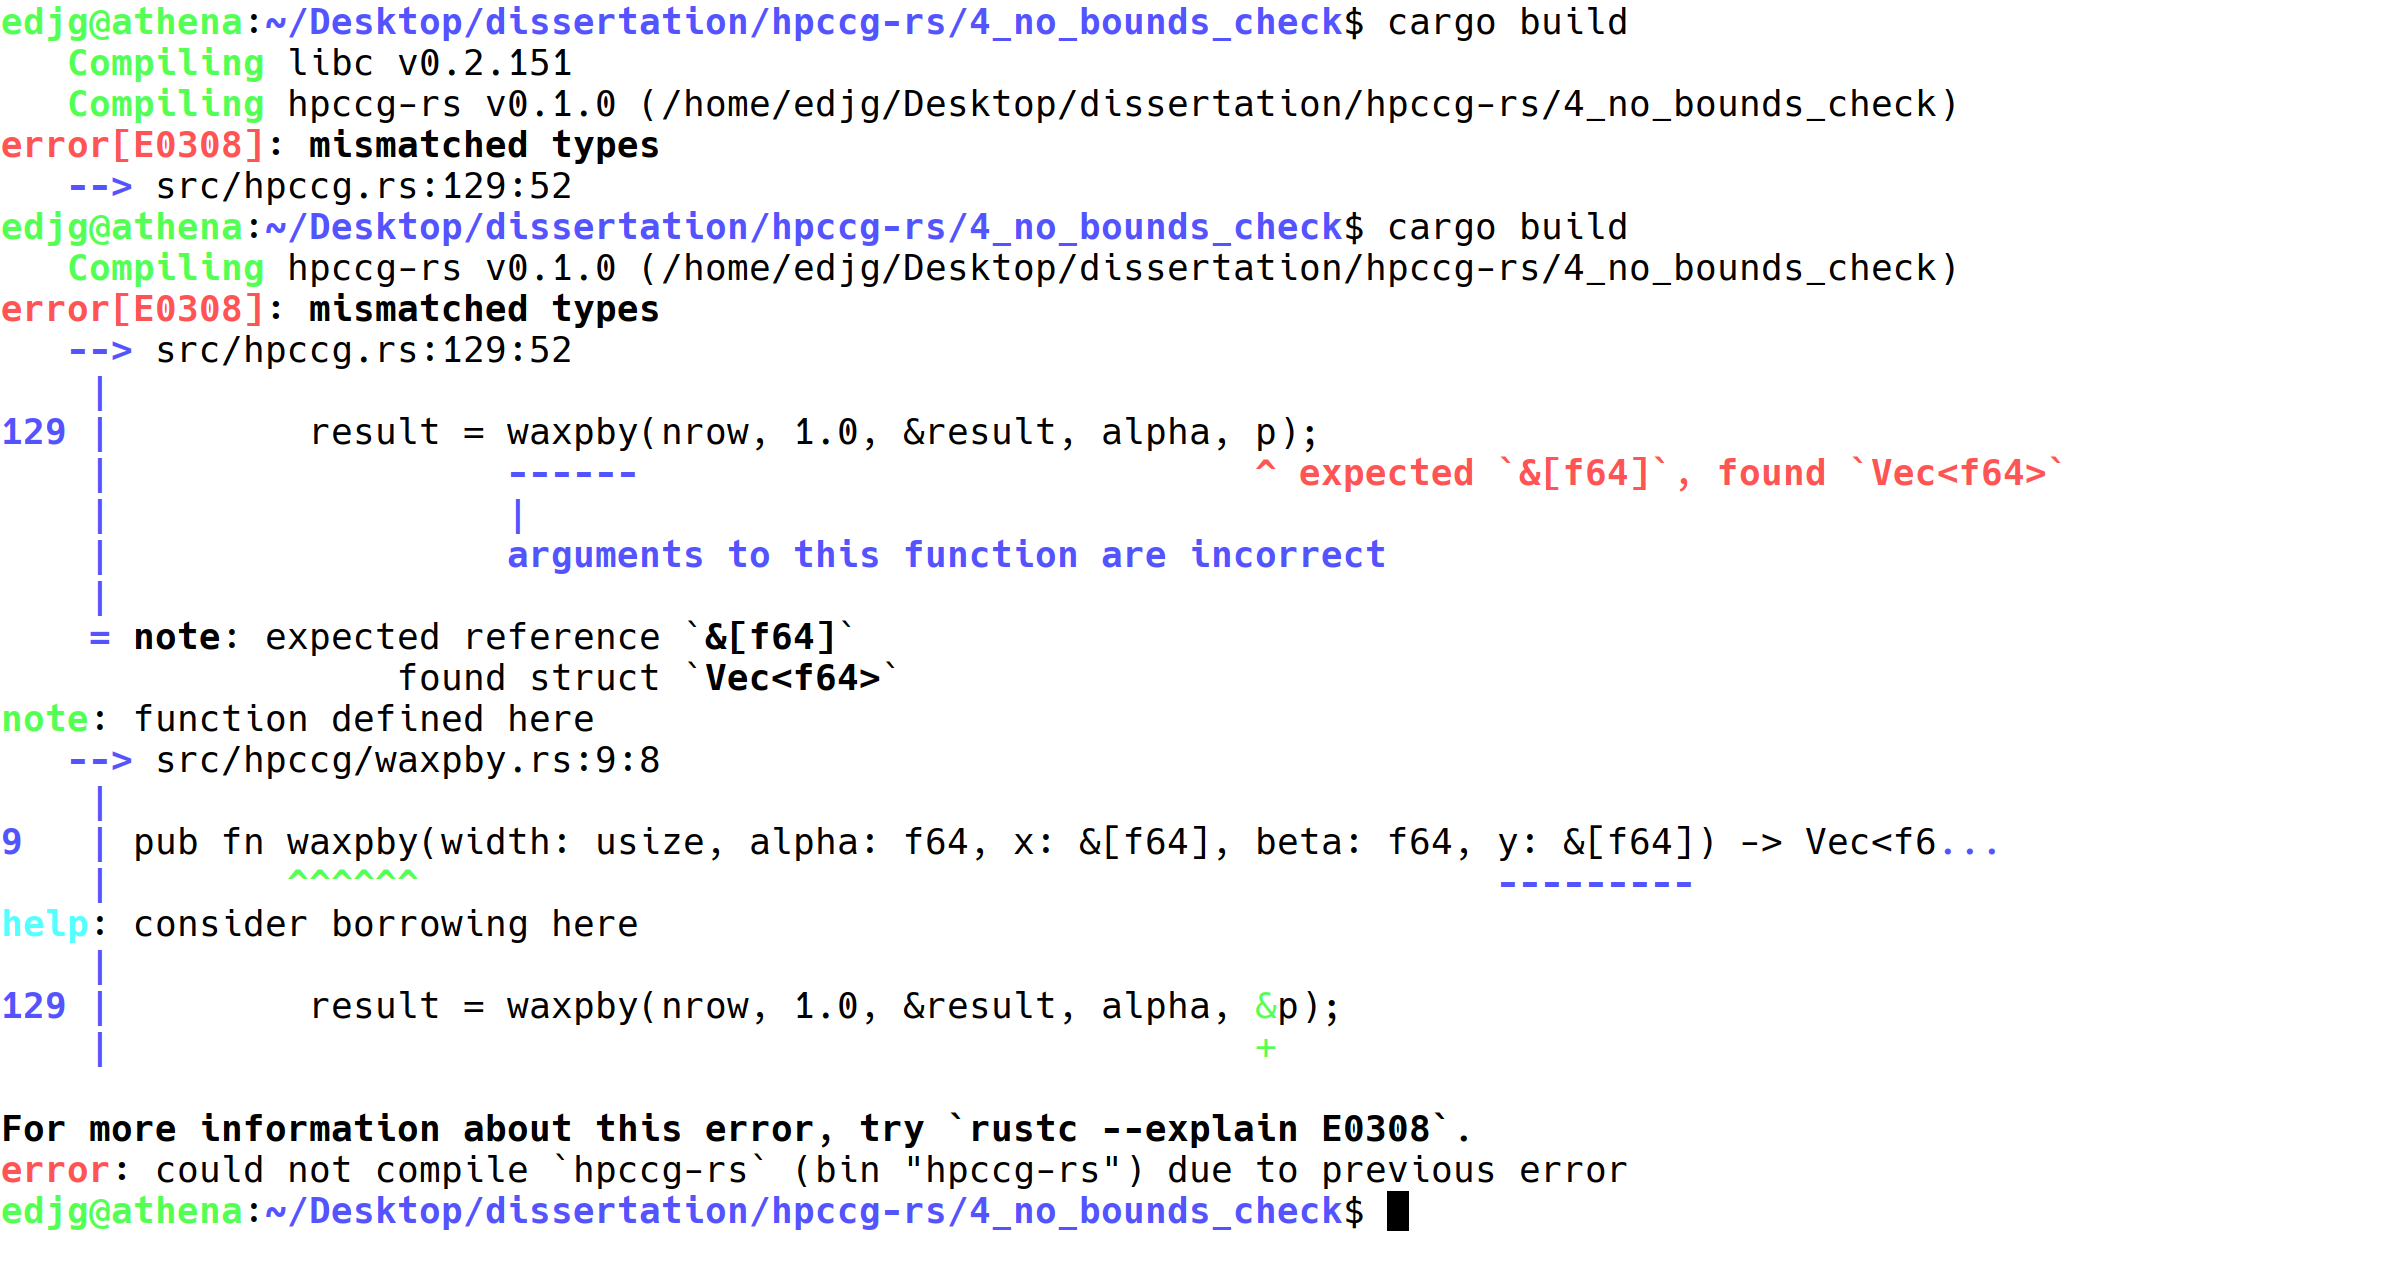
\includegraphics[width=0.95\textwidth]{images/2_background/rust_error_messages.png}
    \caption{Example of an error message, including a correct suggestion to fix it, generated by Rust as a result of a missing \mintinline{rust}{&} required to borrow the value.}
    \label{fig:rust_error_messages}
\end{figure}

On top of this, Rust provides a canonical auto-formatter called \texttt{rustfmt} \cite{RustlangRustfmt2024}, and a linter called \texttt{clippy} \cite{RustlangRustclippy2024}, which are a key component of modern development best practices. This contrasts C++, where various different, often contradictory lint and auto-format standards exist. This means that developers have to make the decision to pick one, rather than just using the canonical one. Finally, Rust provides a package manager called \texttt{cargo} \cite{RustlangCargo2024}, and a package repository called \textit{crates.io} \cite{CratesIoRust}. These allow the Rust community to share packages,
%referred to as crates, % These are not technically the same thing
to extend the functionality of Rust beyond the base language. As a result of this, despite its comparatively young age, Rust has a thriving ecosystem of packages for many tasks. This again contrasts C++, which does not have a canonical package manager, with programmers being split across \texttt{conan} \cite{ConanioConan2024}, \texttt{vcpkg} \cite{MicrosoftVcpkg2024}, domain-specific tools like \texttt{spack} \cite{gamblin2015spack}, and manual installation through header files, causing fragmentation of the package ecosystem.

\subsection{Widespread adoption}
\label{ssec:rust-adoption}

Efforts to adopt Rust in security sensitive parts of existing products, such as parsers for untrusted inputs \cite{OxidationMozillaWiki}, have existed for many years. For example, the first production code example of Mozilla's Oxidation effort to ``integrat[e] Rust code in and around Firefox'' was a MP4 metadata parser in Firefox 48 \cite{OxidationMozillaWiki}, released in 2016. However, in recent years these efforts have become far more widespread, for example Google introducing first-class Rust support for Android development in 2021, motivated by its memory safe properties \cite{RustAndroidPlatform}.

Even in the past two months at the time of writing, there have been widely reported moves towards Rust adoption. Firstly, the White House Office of the National Cyber Director publishing a press release ``Future Software Should Be Memory Safe'', encouraging developers to adopt memory safe languages, such as Rust for systems programming applications, to ``to reduce the attack surface in cyberspace'' as a matter of national security \cite{PressReleaseFuture2024}. In addition to this, Google pledged one million dollars to improve Rust's interoperability with C++, including through tooling such as \texttt{autocxx} \cite{GoogleAutocxx2024} and \texttt{bindgen} \cite{RustlangRustbindgen2024}. In the course of this project, the author made an open source contribution to \texttt{autocxx} to unblock an issue around the use of arrays \cite{goodmanAddIntegrationTests}, a common task in \acrshort{HPC}. This is discussed in more detail in section \ref{sec:open-source-work}.






\section{High performance computing}
\label{sec:hpc}

This background to \acrshort{HPC} will address recent trends in hardware design, and how they impact modern approaches to writing highly performant software. It will then address the Mantevo project, giving a brief history and linking its motivation to software approaches. Finally, it will discuss HPCCG, a \acrshort{mini-app} in the Mantevo project, and the target of the translation effort in this project.

\subsection{Recent trends in hardware design}
\label{ssec:hardware-design-trends}

In the early 2010s, physical limitations began to change how computer hardware was designed. Before this point, performance gains in hardware could be guaranteed by increasing clock speeds. However, as shown in Figure \ref{fig:scaling-trends-transistor-clock}, power limitations heralded the so-called ``death of CPU frequency scaling'', marked by Intel's cancellation of the 4GHz CPU project in 2004 \cite{markovLimitsFundamentalLimits2014}.

% TODO: Check rules about replicating diagrams from paper with correct attribution
\begin{figure}[H]
    \centering
    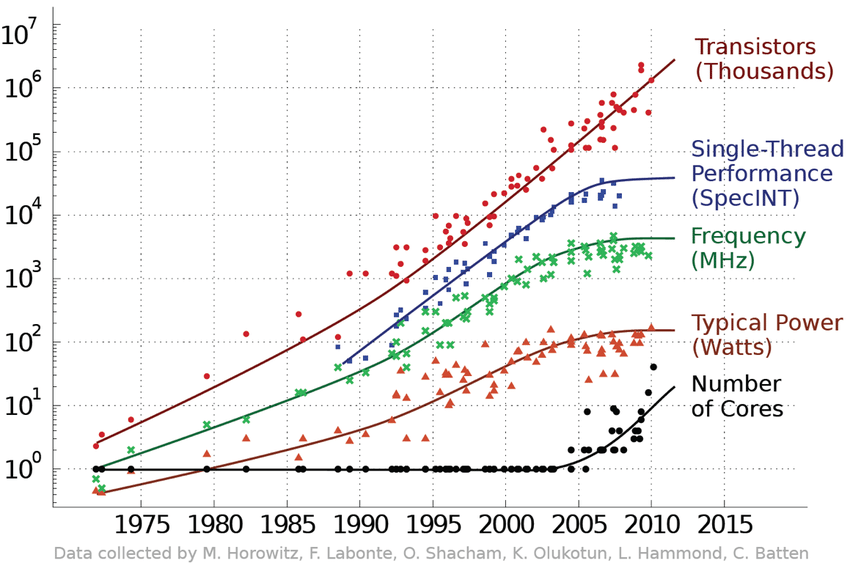
\includegraphics[width=0.75\textwidth]{images/2_background/1-Trends-in-transistor-count-performance-core-count-and-power-over-the-past-decades.png}
    \caption{``Trends in transistor count, performance, core count and power over the past decades'', reproduced from Chao Chen's ``Energy-efficient electrical and silicon-photonic networks in manycore systems'' \cite{chenEnergyefficientElectricalSiliconphotonic2014}.}
    \label{fig:scaling-trends-transistor-clock}
\end{figure}

As a result of this, the 2013 Mantevo paper notes that ``future performance gains come almost solely from running sets of instructions concurrently'' \cite{heroux2013mantevo}. This can be seen in Figure \ref{fig:scaling-trends-transistor-clock} as the increase in prevalence of multicore processors for parallel execution. There are some mechanisms which allow this to be implemented transparently to the programmer in hardware, such as instruction-level parallelism through superscalar processing and out-of-order execution \cite{pattersonHennessyComputerOrganisationArchitecture}, or vectorisation for SIMD processing \cite{pattersonHennessyComputerOrganisationArchitecture}. However, these performance gains begin to be curtailed by data hazards inherent to the software being executed \cite{shahhoseini1999achieving}, along with physical limitations to silicon footprint for a single CPU. As a result of this, parallelism approaches which are not transparent to the programmer are required for further performance increases.

\subsection{Shared memory parallelism}
\label{ssec:shared-memory-paralellism}

Shared memory parallelism refers to dividing work between multiple threads or processes, which all have access to a common memory architecture \cite{SharedMemoryParallelism}. Threads can be defined as ``basic units to which the operating system allocates processor time'' \cite{karl-bridge-microsoftProcessesThreadsWin322021}. In machines with multiple processors in a shared memory architecture, multiple threads can be executed in parallel. When the number of threads exceeds the number of logical processors, the operating system scheduler will interleave the threads to allow concurrent execution. Programs running workloads in parallel on a single machine typically use multiple threads to achieve this parallel execution. Multi-threading for shared memory parallelism can be implemented manually using thread and synchronisation primitives, such as those provided by \texttt{pthread} \cite{nichols1996pthreads}. However, frameworks such as OpenMP \cite{dagumOpenMPIndustryStandard1998} provide a convenient API for writing parallel programs, including compiler directives for FORTRAN and C/C++ which facilitate adding shared memory parallelism to code.

The OpenMP API is designed to make it easy for programmers to leverage parallelism in common programming scenarios, such as iteration. Listings \ref{listing:cpp-ddot}, \ref{listing:cpp-ddot-openmp-race}, and \ref{listing:cpp-ddot-openmp-reduction} provide a simple example of an application of OpenMP to parallelise an implementation of the dot product operation.

\begin{code}
    %TC:ignore
    \begin{minted}{c++}
        double dot_product (
            int n, double* x, double* y
        ) {
            double result = 0.0;
            for (int i = 0; i < n; i++) {
                result += x[i] * y[i];
            }
            return result;
        }
    \end{minted}
    %TC:endignore
    \caption{C++ function implementing the dot product operation on two arrays.}
    \label{listing:cpp-ddot}
\end{code}

\begin{code}
    %TC:ignore
    \begin{minted}{c++}
        double dot_product (
            int n, double* x, double* y
        ) {
            double result = 0.0;
        #pragma omp parallel for
            for (int i = 0; i < n; i++) {
                result += x[i] * y[i];
            }
            return result;
        }
    \end{minted}
    %TC:endignore
    \caption{C++ function using OpenMP to parallelise the dot product operation, containing a race condition.}
    \label{listing:cpp-ddot-openmp-race}
\end{code}

In Figure \ref{listing:cpp-ddot-openmp-race}, we can see the application of the OpenMP pragma \mintinline[breaklines]{c++}{#pragma omp parallel for} on line 5. This demonstrates how intuitive and readable the OpenMP API is, achieving in one line what would take many lines of code to manually implement using \texttt{pthread} primitives. However, Listing \ref{listing:cpp-ddot-openmp-race} contains a data race. On line 7, multiple threads may concurrently increment the result, which is not an atomic operation. This may lead to the program missing array cells from the sum, making the result unreliable.

\begin{code}
    %TC:ignore
    \begin{minted}{c++}
        double dot_product (
            int n, double* x, double* y
        ) {
            double result = 0.0;
        #pragma omp parallel for reduction(+:result)
            for (int i = 0; i < n; i++) {
                result += x[i] * y[i];
            }
            return result;
        }
    \end{minted}
    %TC:endignore
    \caption{C++ function using OpenMP to parallelise the dot product operation, using a reduction to avoid a race condition.}
    \label{listing:cpp-ddot-openmp-reduction}
\end{code}

Listing \ref{listing:cpp-ddot-openmp-reduction} shows how this can be simply mitigated by using an OpenMP reduction, which avoids this issue by maintaining local copies of the result across threads, then combining them at the end. However, this shows how susceptible even simple parallel programs can be to errors which are difficult to debug. As discussed in section \ref{ssec:rust-fearless-concurrency}, Rust provides guarantees against this category of undefined behaviour, motivating its use in \acrshort{HPC} applications, which often rely heavily on multi-threading.

The multi-threading approach to parallel is very effective for single machines running small or medium-sized programs. However, it is dependent on the machine it is executing having a shared memory architecture, so cannot scale beyond running on a single machine to clusters of computers. As a result of this, different approaches are required to aggregate together the work done by machines within a compute cluster with a distributed memory architecture.

\subsection{Distributed memory parallelism}
\label{ssec:distributed-memory-paralellism}

Distributed memory parallelism refers to dividing work across ``a computing system in which each processor has its memory'' \cite{pardo2021modeling}. A common approach to implement this is a message passing across a high-speed network connection. MPI, an initialism for Message Passing Interface, is a standard first proposed in 1993 which defined a communication protocol for exchanging data between ``MIMD distributed memory concurrent computers'' \cite{thempiforumMPIMessagePassing1993}. Two pieces of key terminology in MPI are ``rank'' and ``size''. Size refers to the number of distributed processors being used to execute the program, and rank the unique index of the processor an instance of code is executing on -- bounded between $0$ and $size-1$. MPI allows the concurrent execution of programs across many distributed processors, with each individual program rank running independently, but able to communicate with other ranks via message passing.

There are multiple implementations of the MPI standard, such as OpenMPI \cite{gabriel2004open} and MPICH \cite{gropp1996user}. These provide the functionality defined by the MPI standard for languages such as C++, FORTRAN, and Java. The MPI API is more complex than OpenMP, without the convenient compiler directives for parallelising loops, instead requiring more manual control over the way in which work is distributed. However, this provides the commensurate benefit of the ability to precisely control how data is shared, and allows it to operate over a distributed memory architecture.

Again taking the example of the dot product operation shown in Listing \ref{listing:cpp-ddot}, Listing \ref{listing:cpp-ddot-mpi} shows how MPI can be used to distribute the operation across a many ranks, allowing it to leverage parallelism on a distributed memory architecture.

\begin{code}
    %TC:ignore
    \begin{minted}{c++}
        #include <mpi.h>
        
        double dot_product (
            int n, double* x, double* y
        ) {
            // Manually split the array across the ranks
            int size, rank;
            MPI_Comm_size(MPI_COMM_WORLD, &size);
            MPI_Comm_rank(MPI_COMM_WORLD, &rank);
            int offset = ((n / size) * rank);
            int length = (rank != size - 1) ? length / size : length - offset;
        
            // Calculate the dot product for the rank's array slice
            double local_result = 0.0;
            for (int i = offset; i < offset + length; i++) {
                local_result += x[i] * y[i];
            }
        
            // Reduce the result across all the ranks
            double result = 0.0;
            MPI_Allreduce(&local_result, &result, 1, MPI_DOUBLE, MPI_SUM, MPI_COMM_WORLD);
            return result;
        }
    \end{minted}
    %TC:endignore
    \caption{C++ function using MPI to parallelise the dot product operation.}
    \label{listing:cpp-ddot-mpi}
\end{code}

Even in this simple code snippet, we can see the additional programmer effort required to use MPI over OpenMP. Lines 6 to 11 of Listing \ref{listing:cpp-ddot-mpi} manually split up the array to the ranks, whereas the OpenMP compiler directive does this automatically. The \mintinline{rust}{MPI_Allreduce} command on line 21 sends messages containing the local result to be reduced together with the \mintinline{rust}{MPI_SUM} operation to calculate the global result, which is the transmitted back as a message to all the ranks.

\subsection{Performance portability frameworks}
\label{ssec:performance-portability-frameworks}

There also exist portability frameworks, such as Kokkos \cite{edwardsKokkosEnablingPerformance2013} and RAJA \cite{RAJAPortabilitySuite}, which provide an abstraction over many parallelism techniques to improve software portability. This reduces the programmer effort to write software which is highly performant across different hardware, but can incur a performance cost. As with OpenMP and MPI, taking the example of the dot product operation shown in Listing \ref{listing:cpp-ddot}, an implementation of the same function using Kokkos for parallel execution is shown in Listing \ref{listing:cpp-ddot-kokkos}.

\begin{code}
    %TC:ignore
    \begin{minted}{c++}
        #include <Kokkos_Core.hpp>
        
        double dot_product (
            int n, double* x, double* y
        ) {
            double result = 0.0;
            Kokkos::parallel_reduce(
                n,
                KOKKOS_LAMBDA(const int i, double& ksum) {
                     ksum += x[i] * y[i];
                },
                result
            );
            return result;
        }
    \end{minted}
    %TC:endignore
    \caption{C++ function using OpenMP to parallelise the dot product operation, using a reduction to avoid a race condition.}
    \label{listing:cpp-ddot-kokkos}
\end{code}

Kokkos is designed to be ``hardware agnostic'', providing an abstraction for writing performant code which can run on across CPUs and GPUs from a variety of hardware vendors \cite{KokkosEcosystem}. As discussed in the later section \ref{ssec:p3hpc}, this provides both productivity and portability for the programmer, as this abstraction means they can be less concerned about compatibility across hardware. However, this can come at a performance cost, as the abstraction may not be able to compile to be as performant as hand-optimised code. The prominence of Kokkos in the \acrshort{HPC} space is encouraging for the suitability of Rust for the same space, as it means that programmers are willing to make sacrifices in performance for commensurate improvements to other aspects of software development, such as productivity and portability.

Since these mechanisms to leverage hardware for performance improvements are not transparent to the programmer, hardware-software co-design, defined by the 2013 Mantevo paper as ``collaborative simultaneous development of all system components'' \cite{heroux2013mantevo} became essential. As a result of this, new techniques were required for the effective co-design of high-performance systems.

\subsection{Mini-apps and the Mantevo Suite}
\label{ssec:miniapps-mantevo}

The Mantevo project at Sandia National Labs pioneered the concept of \acrshort{mini-app}s as a tool for hardware-software co-design, publishing the Mantevo Suite in late 2012 as a collection of full-featured \acrshort{mini-app}s for this purpose. It defines \acrshort{mini-app}s as ``Small software programs [...] whose performance characteristics model full-scale applications, yet require only a fraction of the lines of code, making [them] easier to study, design, and re-write'' \cite{heroux2013mantevo}.

The use of \acrshort{mini-app}s makes hardware-software co-design for large, complex applications possible. This is because they can be used in place of the production application whose performance they model when making very early design decisions, without incurring the cost of massive complexity of the production application. Traditionally, \acrshort{mini-app}s have been used to predict the performance of production applications on new hardware. However, this concept can be inverted to instead use \acrshort{mini-app}s to predict the performance on the underlying software stack, for example the programming language of implementation.

\subsection{HPCCG}
\label{ssec:hpccg}

HPCCG is an initialism for ``High Performance Computing Conjugate Gradients'', and is ``the original Mantevo mini-app'' \cite{herouxHPCCGSolverPackage2007}. It is designed to be ``the best approximation to an unstructured implicit finite element or finite volume application in 800 lines or fewer.'' \cite{PackagesMantevo}. This short length, along with its simple build system, and support for OpenMP and MPI with no other dependencies made it a good choice for translation to Rust. A full description of the process leading to the selection of HPCCG is described in Appendix \ref{sec:miniapp-selection}.

It is based on the iterative method of gradient descent for conjugate gradients first proposed by Hestnes and Steifel in 1952\cite{hestenesMethodsConjugateGradients1952}, who researched it and wrote an implementation for the contemporary Z4 processor. This process can be used to model, and hence visualise, pressure dissipation over time in a three-dimensional mesh as shown in Figure \ref{fig:acacgs_silo_output}.

\begin{figure}[H]
    \centering
    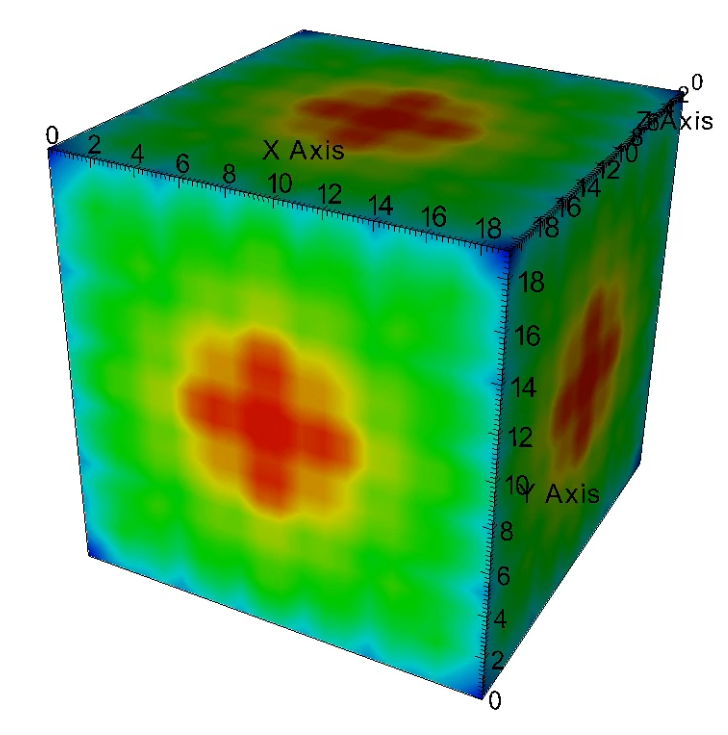
\includegraphics[width=0.5\textwidth]{images/2_background/acacgs_silo_output.png}
    \caption{VisIt visualisation from ACACGS, a C translation of HPCCG by Dr Richard Kirk which is used in the CS257 Advanced Computer Architecture coursework.}
    \label{fig:acacgs_silo_output}
\end{figure}

There are three main operations in this iterative method of conjugate gradients: calculating a vector dot product, pairwise summation of two scaled vectors, and calculating the product of a sparse matrix and a vector. Of the three operations, the third operation is responsible for most of the floating point operations, and consequently the majority of the runtime. This is because calculating sparse matrix-vector products requires larger and more complex data structures to efficiently represent sparse matrices, rather than just vectors.

Sparse matrix-vector products are a common workload in \acrshort{HPC}, and remain an active field of research, with Lane and Booth describing them as ``one of the most important kernels in high-performance computing'' \cite{laneHeterogeneousSparseMatrixVector2023}. This means that the performance characteristics of HPCCG, which are dominated by this kernel, are representative of many large applications. Since sparse matrices are ubiquitous in computational tasks, there are well-established data structures to represent them. One of these representations is compressed row storage, often called Yale format, as it was first proposed in the 1977 Yale Sparse Matrix Package report \cite{eisenstat1977yale}.

\subsection{Performance, Productivity, and Portability}
\label{ssec:p3hpc}

In the real world, \acrshort{HPC} projects are constrained by budget. Since supercomputers are extraordinarily expensive, it is easy to assume that the dominant effect on project cost is performance, as more performant software requires less time on the supercomputer, which costs money. However, other aspects of software engineering also impact the calculus of the cost of \acrshort{HPC} projects. Engineers are required to build software and maintain the servers for the project, and high-quality engineers capable of undertaking such tasks require high salaries. As a result of this, productivity and portability play a significant role in project cost, as well as raw performance. This fact is confirmed by the existence of the P3HPC conference, standing for ``Performance, Portability, and Productivity in HPC'', which focusses on ``research that addresses the complexities of real-life applications and/or realistic workloads'' \cite{P3HPC}.

% NOTE: THIS IS A KEY PARAGRAPH! IS IT PROMINENT ENOUGH?
Developer productivity plays a key role in \acrshort{HPC} projects. This is because is more productive developers will complete tasks more quickly, so fewer developer hours are required per project. In addition to this, projects with the same number of developers will be completed faster if the developers are more productive. In real projects constrained by budget, these are both clearly desirable outcomes. As a result of this, workflows and methodologies which can augment developer productivity are very beneficial within \acrshort{HPC}. Rust's guarantees of memory and thread safety, its terse syntax, and robust development toolchain all contribute to developer productivity, with fewer lines of code required to express the same functionality, and less time spent debugging.

Portability across hardware architectures is also a key consideration when building software for \acrshort{HPC} systems. Supercomputers are not homogeneous in architecture, with Intel, AMD, and Cray all being common platforms. Performance characteristics of software across architectures are difficult to predict, with architectural choices such as cache size deeply impacting performance of certain workloads. As a result of this, techniques to build software which is portable across many systems are very desirable.

% NOTE: Is this consistent tense?
As a result of this, this project will take a holistic view of software development for \acrshort{HPC}, assessing not only the raw performance of Rust, but also taking into context its effects on developer productivity, and its portability across different hardware architectures. In addition to this, developer tooling will be built to enhance the productivity of engineers in aspects of the translation workflow identified as viable for augmentation by tooling.


\section{Literature review}
\label{sec:literature-review}

Rust's popularity has led to academic investigations of its suitability for many tasks, despite it being a relatively young language. This literature review will start with a paper discussing the overall landscape of language performance for \acrshort{HPC}, comparing a single workload across 10 languages. Then, it will critically evaluate a number of performance analyses of Rust in \acrshort{HPC}, in order to cover a variety of techniques, from serial to highly parallel, and a variety of benchmark types, from algorithm snippets to full codebases. This project differs from existing work, as no existing analysis covers the implementation of an established \acrshort{mini-app} to highly-parallel clustered compute, and it will include an assessment of practical suitability beyond just performance measurements. Furthermore, it will go beyond comparison to build tooling and workflows to directly improve any issues identified during this assessment.

\subsection{Benchmarking the Parallel 1D Heat Equation Solver}
\label{ssec:diehl-et-al}

% Benchmarking the Parallel 1D Heat Equation Solver in Chapel, Charm++, C++, HPX, Go, Julia, Python, Rust, Swift, and Java
% https://github.com/diehlpk/async_heat_equation/tree/main
Diehl et al. present a general overview of the landscape of language performance for a representative \acrshort{HPC} workload in their paper ``Benchmarking the Parallel 1D Heat Equation Solver in Chapel, Charm++, C++, HPX, Go, Julia, Python, Rust, Swift, and Java'' \cite{diehlBenchmarkingParallel1D2023}. This paper selects a 1D heat diffusion solver algorithm to implement, as it uses block-structured meshes, which are commonly used in \acrshort{HPC} applications. It then goes on to qualitatively discuss the experience of implementing the algorithm in the different languages, and suggests a quantitative metric for assessing implementation difficulty, the \acrfull{COCOMO} \cite{boehm1995cost}. Finally, it benchmarks these implementations across three different hardware architectures, and constructs a plot comparing program runtime against its metric for implementation difficulty, duplicated in Figure \ref{fig:1d_heat_results}. The paper concludes that ``one solution does not fit all'', but names C++ as a common choice as it is both popular and performant, whilst noting Rust's ``innovative ideas will make it ideally suited for many applications''.

\begin{figure}[H]
    \centering
    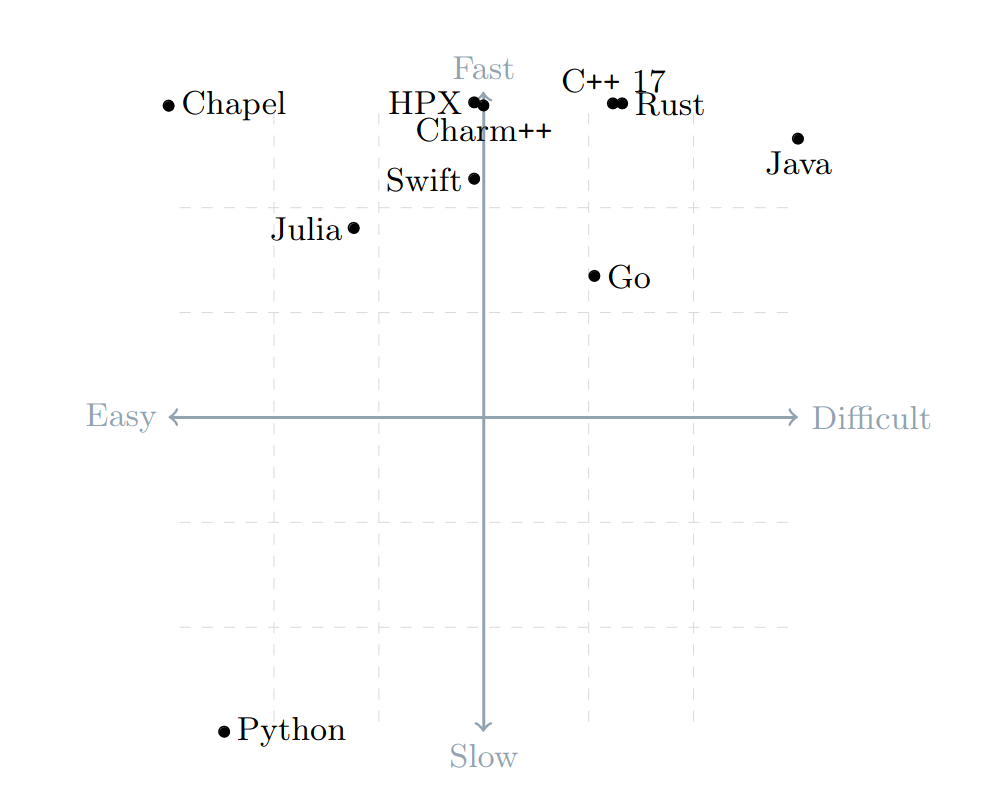
\includegraphics[width=0.75\textwidth]{images/2_background/1d_heat_results.png}
    \caption{``Two-dimensional classification using the computational time and the \acrshort{COCOMO} model [sic]'', reproduced from Diehl et al.'s paper \cite{diehlBenchmarkingParallel1D2023}.}
    \label{fig:1d_heat_results}
    % TODO: Check paper website for permission to reproduce
\end{figure}

Diehl et al. provide a strong empirical analysis of the landscape of languages in the context of \acrshort{HPC}, and provide source code as a GitHub repository \cite{diehlInitialRelease2023} along with naming the multiple processors used for benchmarking, allowing reproducibility of their results. However, they explicitly do not provide their measurements other than in plots, choosing ``not to name a winner with respect to speed''. Additionally, they do not provide details on their test methodology beyond naming the metrics measured and the names of hardware they used. Providing concrete results, along with a more specific methodology such as thread counts, memory size, or number of experiment re-runs would provide much more confidence in the conclusions drawn. Finally, their future work notes that the selected algorithm only runs on a single CPU, and as such does not explore using MPI for distributing compute over a clustered resource, nor does it explore GPU support using a language like CUDA, nor abstractions layers like Kokkos.

\subsection{Rust language for supercomputing applications}
\label{ssec:bychkov-nikolskiy}

% Rust language for supercomputing applications
% Serial, parallel, and MPI - but on non-standard small code snippet benchmarks. Present but flawed methodology.
Bychkov and Nikolskiy examine the readiness of the Rust language for supercomputer applications in their paper ``Rust Language for Supercomputing Applications'' \cite{bychkovRustLanguageSupercomputing2021}. The main contribution of this paper is the critical comparison of Rust and C++ over a set of benchmarks. The first benchmark characterises serial performance via a handwritten implementation of the matrix multiplication algorithm in each language. The authors note that naive rust implementations perform poorly in comparison with C++, but writing idiomatic Rust and leveraging optimisation techniques can close this performance gap. A later benchmark characterises the performance of shared-memory parallelism via multi-threading, using OpenMP and \texttt{rayon} for C++ and Rust respectively, finding that both have similar performance and scaling characteristics on the selected benchmark. The final benchmark compares the C++ native implementation of the MPI specification with the Rust bindings to it. The paper notes that since the Rust bindings are memory safe and leverage the rich type system, they provide many desirable properties such as guarantees of memory and thread safety and minimising boilerplate. The paper concludes that Rust is competitive to C++ for the benchmarks it explored, and that there is sufficient support for writing parallel code.

Bychkov and Nikolskiy present an empirical analysis directly comparing Rust and C++ only across a number of different benchmarks, contrasting Diehl et al. by providing a more specific analysis rather than a general view of the landscape. The paper gives fair reproducibility of results by clearly stating the benchmarking methodology, including machine specifications, operating system, and compiler versions. However, the choice of methodology for non-clustered machines has weaknesses. Notably, the benchmarks were run on a laptop, which can introduce noise into performance measurements if other applications are running in the background. Furthermore, the benchmarks are run under Windows Subsystem for Linux, a virtualisation technology, which significantly impacts program performance and may not be comparable to benchmarks run on unvirtualised systems. Finally, although the MPI benchmarks are run on a compute cluster which avoids the previously itemised issues, the results appear erroneous, with the authors noting ``we discovered [an] unexpected difference between Rust and C++ performance in MPI latency benchmarks'', and stating intent to re-validate the results.

% If needed, perhaps later... Higher quality paper than Bychkov and Nikolskiy, so consider replacing
% Rust programming language in the high-performance computing environment
% Rayon + MPI implementation of code snippet, run data but no source code

\subsection{Performance vs Programming Effort between Rust and C on Multicore Architectures}
\label{ssec:costanzo-et-al}

% Performance vs Programming Effort between Rust and C on Multicore Architectures: Case Study in N-Body
% https://github.com/ManuelCostanzo/Gravitational_N_Bodies_Rust (250 lines of rust)
Costanzo et al. investigate the difference between both performance and programming effort between Rust and C for N-body simulations in their paper ``Performance vs Programming Effort between Rust and C on Multicore Architectures: Case Study in N-Body'' \cite{costanzoPerformanceVsProgramming2021}. The paper introduces Rust as a programming language which may be suitable for \acrshort{HPC} due to its ownership model avoiding the need for garbage collection, and its strong support for shared-memory parallelism. It then discusses the implementation and performance optimisation of C and Rust to the gravitational n-body problem, a simple and well-known computational task. It finally compares the both the performance and programming effort of the C and Rust implementations. The paper concludes that Rust is either equally performant or slightly ($1.18\times$) slower depending on the data type precision, but that this may change with future compiler updates, and Rust requires a lower programming both in terms of lines of code and ease of parallelisation.

Costanzo et al. provide a very compelling empirical analysis comparing Rust and C++, which differs from Bychkov and Nikolskiy by considering both the practical implications of programming effort, and making the comparison on a representative code sample rather than simple benchmarks. However, the paper does not consider highly-parallel clustered compute using technologies such as MPI. The paper provides a discussion of practical techniques for writing performant Rust beyond threading, including use of SIMD intrinsics and custom memory allocators, along with a compelling and unbiased performance analysis of Rust and C++.


\subsection{Emerging technologies, Rust in HPC}
\label{ssec:moran-bull}

% Emerging technologies, Rust in HPC
% Parallel only implementation for non-standard very small full application for C++ and Fortran, good methodology. Poor Rust implementation
% https://github.com/lmoran94/eurocc_cfd (112 lines of Rust)
Moran and Bull \cite{moranEmergingTechnologiesRust2023} investigate the performance of Rust as compared with C++ and FORTRAN on computational fluid dynamics problems in their technical report ``Emerging Technologies: Rust in HPC'' \cite{moranEmergingTechnologiesRust2023}. As with Costanzo et al., Rust is introduced as a programming language which may be suitable for HPC, and the selected problem domain is explained as representative of common \acrshort{HPC} workloads. The paper goes on to benchmark Rust implementations of the problem on a HPC system, and compare them to C++ and FORTRAN implementations. The paper concludes that Rust is slower than C++ and FORTRAN for parallel workloads.

Moran and Bull present a similar empirical analysis to Costanzo et al., comparing a small custom codebase which is representative of \acrshort{HPC} workloads, but differs by including FORTRAN in its comparisons, along with placing a greater focus on performance analysis and scaling, and less consideration to programming effort. However, Moran and Bull report significantly slower performance, significantly trailing C++ and FORTRAN, which contrasts Costanzo et al.'s findings of Rust being slightly slower or equally performant. Moran and Bull attribute their findings to the Rust compiler's attitude to memory safety.

However, inspecting the source code made public after the publication of the paper \cite{Lmoran94Eurocc_cfdCFD}, it can be seen that the implementation does not leverage all the performance capabilities of Rust. For example, it does not apply all of the optimisation techniques enumerated in Costanzo et al.'s paper. A reader of the paper created an optimised version  \cite{moranPaperFalse} \cite{phazer99HerePlayground2023}, which shows a 50\% performance increase over the paper's implementation by avoiding an extraneous copy operation, bringing Rust's performance closer to C++ and FORTRAN. However, this change makes the comparison against FORTRAN and C++ unfair, as the reference implementations also rely on this extraneous copy operation. A replication trial of the experiments in the paper using the published code is presented in section \ref{ssec:hpc-multibench-replication-study}, as both a demonstration of the utility of the HPC MultiBench tool, and to investigate the difference to Costanzo et al.'s findings.
% In summary, possibly flawed due to bounds checked memory access, but not as flawed as some commentators looking only at the Rust implementation think it is.


% % Towards Safe HPC: Productivity and Performance via Rust Interfaces for a Distributed C++ Actors Library
% % This could be omitted, as they paper is a ``work in progress'' and clearly flawed, and other more interesting papers exist...
% Parrish et al. present a framework for writing parallel programs, including a performance analysis of this framework, in their paper ``Towards Safe HPC: Productivity and Performance via Rust Interfaces for a Distributed C++ Actors Library (Work in Progress) [sic]'' \cite{parrishSafeHPCProductivity2023}. The paper concludes that their ``Rust versions of the original application performed on par with the respective C++ versions''. To support this claim, the paper includes figures showing the performance of Rust and C++ for various kernels, such as the one shown replicated in Figure \ref{fig:actors_bad_histogram}.

% \begin{figure}[H]
%     \centering
%     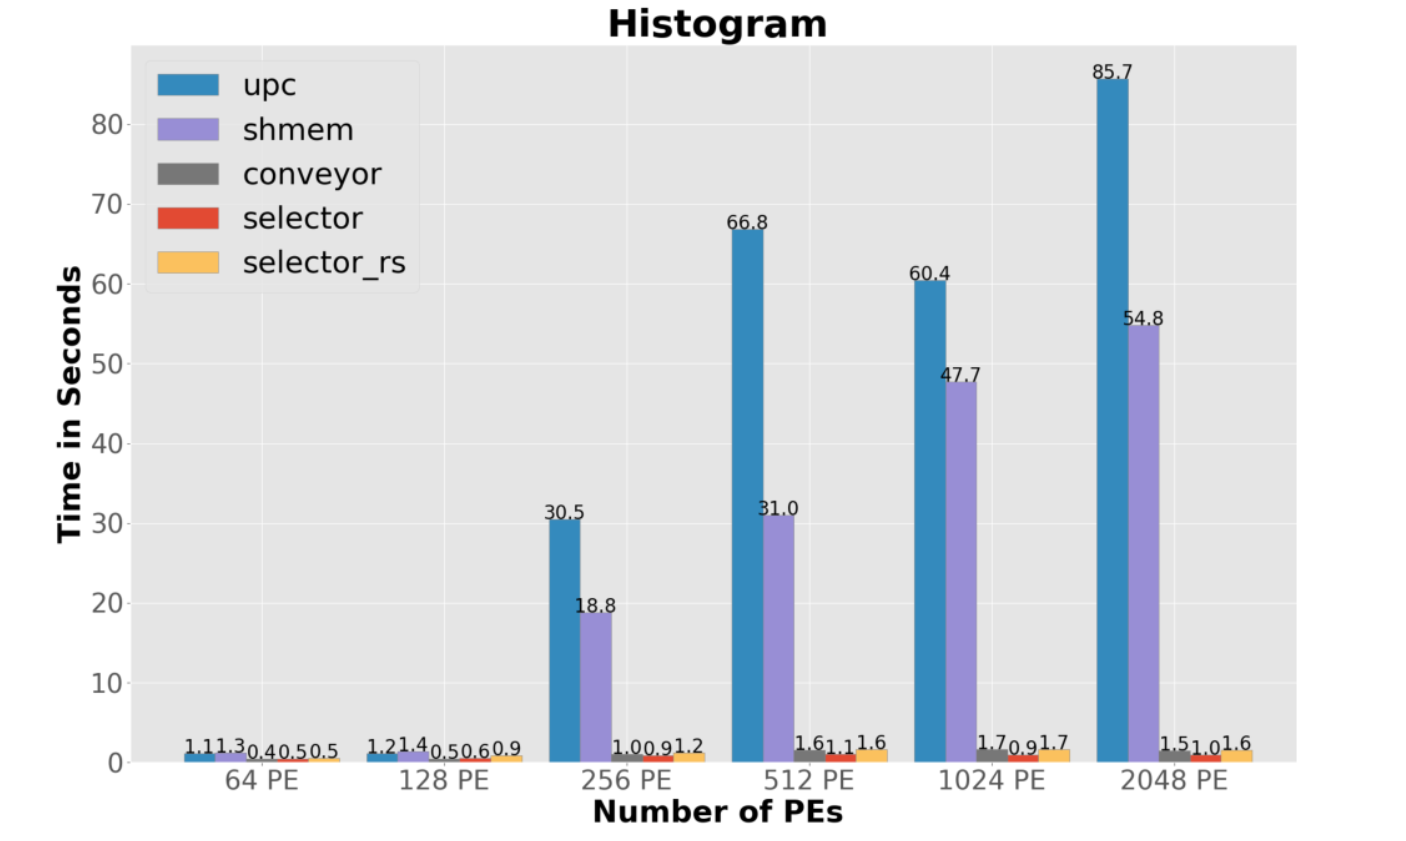
\includegraphics[width=0.75\textwidth]{images/2_background/actors_bad_histogram.png}
%     \caption{The performance of the Histogram kernel across various implementations, reproduced from Appendix A of Parrish et al. \cite{parrishSafeHPCProductivity2023}.}
%     \label{fig:actors_bad_histogram}
%     % TODO: Check paper website for permission to reproduce
% \end{figure}

% However, the data shown in Figure \ref{fig:actors_bad_histogram} does not support the claim that Rust is as performant as C++. The inclusion of the much slower ``upc'' and ``shmem'' implementations skew the scale of the plot so Rust and C++ versions look the same, but in fact by examining the data labels we can see the implementation is on average $1.46\times$ slower for this kernel, which is non-negligibly slower. This aligns with the results of other publications such as Costanzo et al. who observed a $1.18\times$ slowdown, and noted it as such. In the author's opinion, this paper is emblematic of a common problem in literature about the Rust programming language -- the bias held by some that the Rust programming language is better in all respects than other programming languages. Despite the fact that the data in the paper shows that the Rust implementation is slower \ref{fig:actors_bad_histogram}, the data is presented disingenuously in order to draw the conclusion that it is equally performant.

\subsection{Summary of literature}
\label{ssec:literature-summary}

% % Summary
% In summary, there is existing research around the suitability of Rust in High-Performance Computing, which broadly concludes that Rust is slightly slower than C++, but provides other benefits which might mitigate this fact. Some papers, such as Parrish et al. \cite{parrishSafeHPCProductivity2023} over-report the performance of Rust as equal to C++, in spite of the data they present to justify their conclusions. However, other papers, such as Moran and Bull \cite{moranEmergingTechnologiesRust2023}, under-report the performance of Rust as significantly slower than C++, likely due to not fully leveraging possible performance optimisations.
In summary, there is existing research around the suitability of Rust in \acrshort{HPC}, which broadly concludes that Rust is slightly slower than C++, but provides other benefits which might mitigate this. Some papers, such as Moran and Bull \cite{moranEmergingTechnologiesRust2023}, report the performance of Rust as significantly slower than C++. This could be as a result of different computation kernels being less amenable to optimisation, or the authors not fully leveraging performance optimisations possible in Rust.

The existence of publications, such as the ones reviewed above, in this area is compelling that it is a relevant and difficult question to answer. However, there is still space for novel contribution, for example by assessing highly-parallel clustered compute as applied to a standard \acrshort{mini-app}, rather than a simple benchmark or toy example. Furthermore, many existing papers do not focus on reproducibility of results, by omitting the source code, research methodology, or recorded results. Finally, none of the papers provide tooling to assist in the process of translating \acrshort{HPC} codebases, giving a further opportunity for novel contribution.
